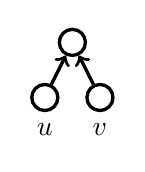
\begin{tikzpicture}[
    scale=0.35,
    line width=1.2pt
]

    % \node at (-3,-5.5) {\(F_1\)};
    
    \node[circle, draw=black, fill=white, label=below:{\(u\)}]
            (p0) at (-4,-4) {};

    \node[circle, draw=black, fill=white, label=below:{\(v\)}]
            (p1) at (-2,-4) {};

    \node[circle, draw=black, fill=white]
        (p2) at (-3,-2) {};
    

    \draw[->] (p0) -- (p2);
    \draw[->] (p1) -- (p2);
\end{tikzpicture}